\documentclass[11pt,letterpaper]{exam}
\usepackage[spanish]{babel}
\usepackage{graphicx}
\usepackage{tabularx}
\usepackage[absolute]{textpos} % Para poner una imagen en posiciones arbitrarias
\usepackage{multirow}
\usepackage{float}
\usepackage{hyperref}
\usepackage[utf8x]{inputenc} 
\usepackage[normalem]{ulem}
\useunder{\uline}{\ul}{}
\usepackage[usenames]{color}
\title{Tarea 2 Métodos Computacionales}
\author{Valeria Martín Hernández}

\date{Mayo 2019}

\begin{document}


\maketitle
\newpage


\section{Ejercicio 2: Transformadas de Fourier}
En el ejercicio de Fourier, debe incluir todas las gráficas y debe explicar lo que observa en las gráficas. Debe en particular describir lo que observa en las gráficas de espectrogramas (tambien llamados time frequency plots). 
\subsection{Signal.dat y signalSuma.dat:}
\subsubsection{Grafica general}
\begin{figure}[H]
    \centering
    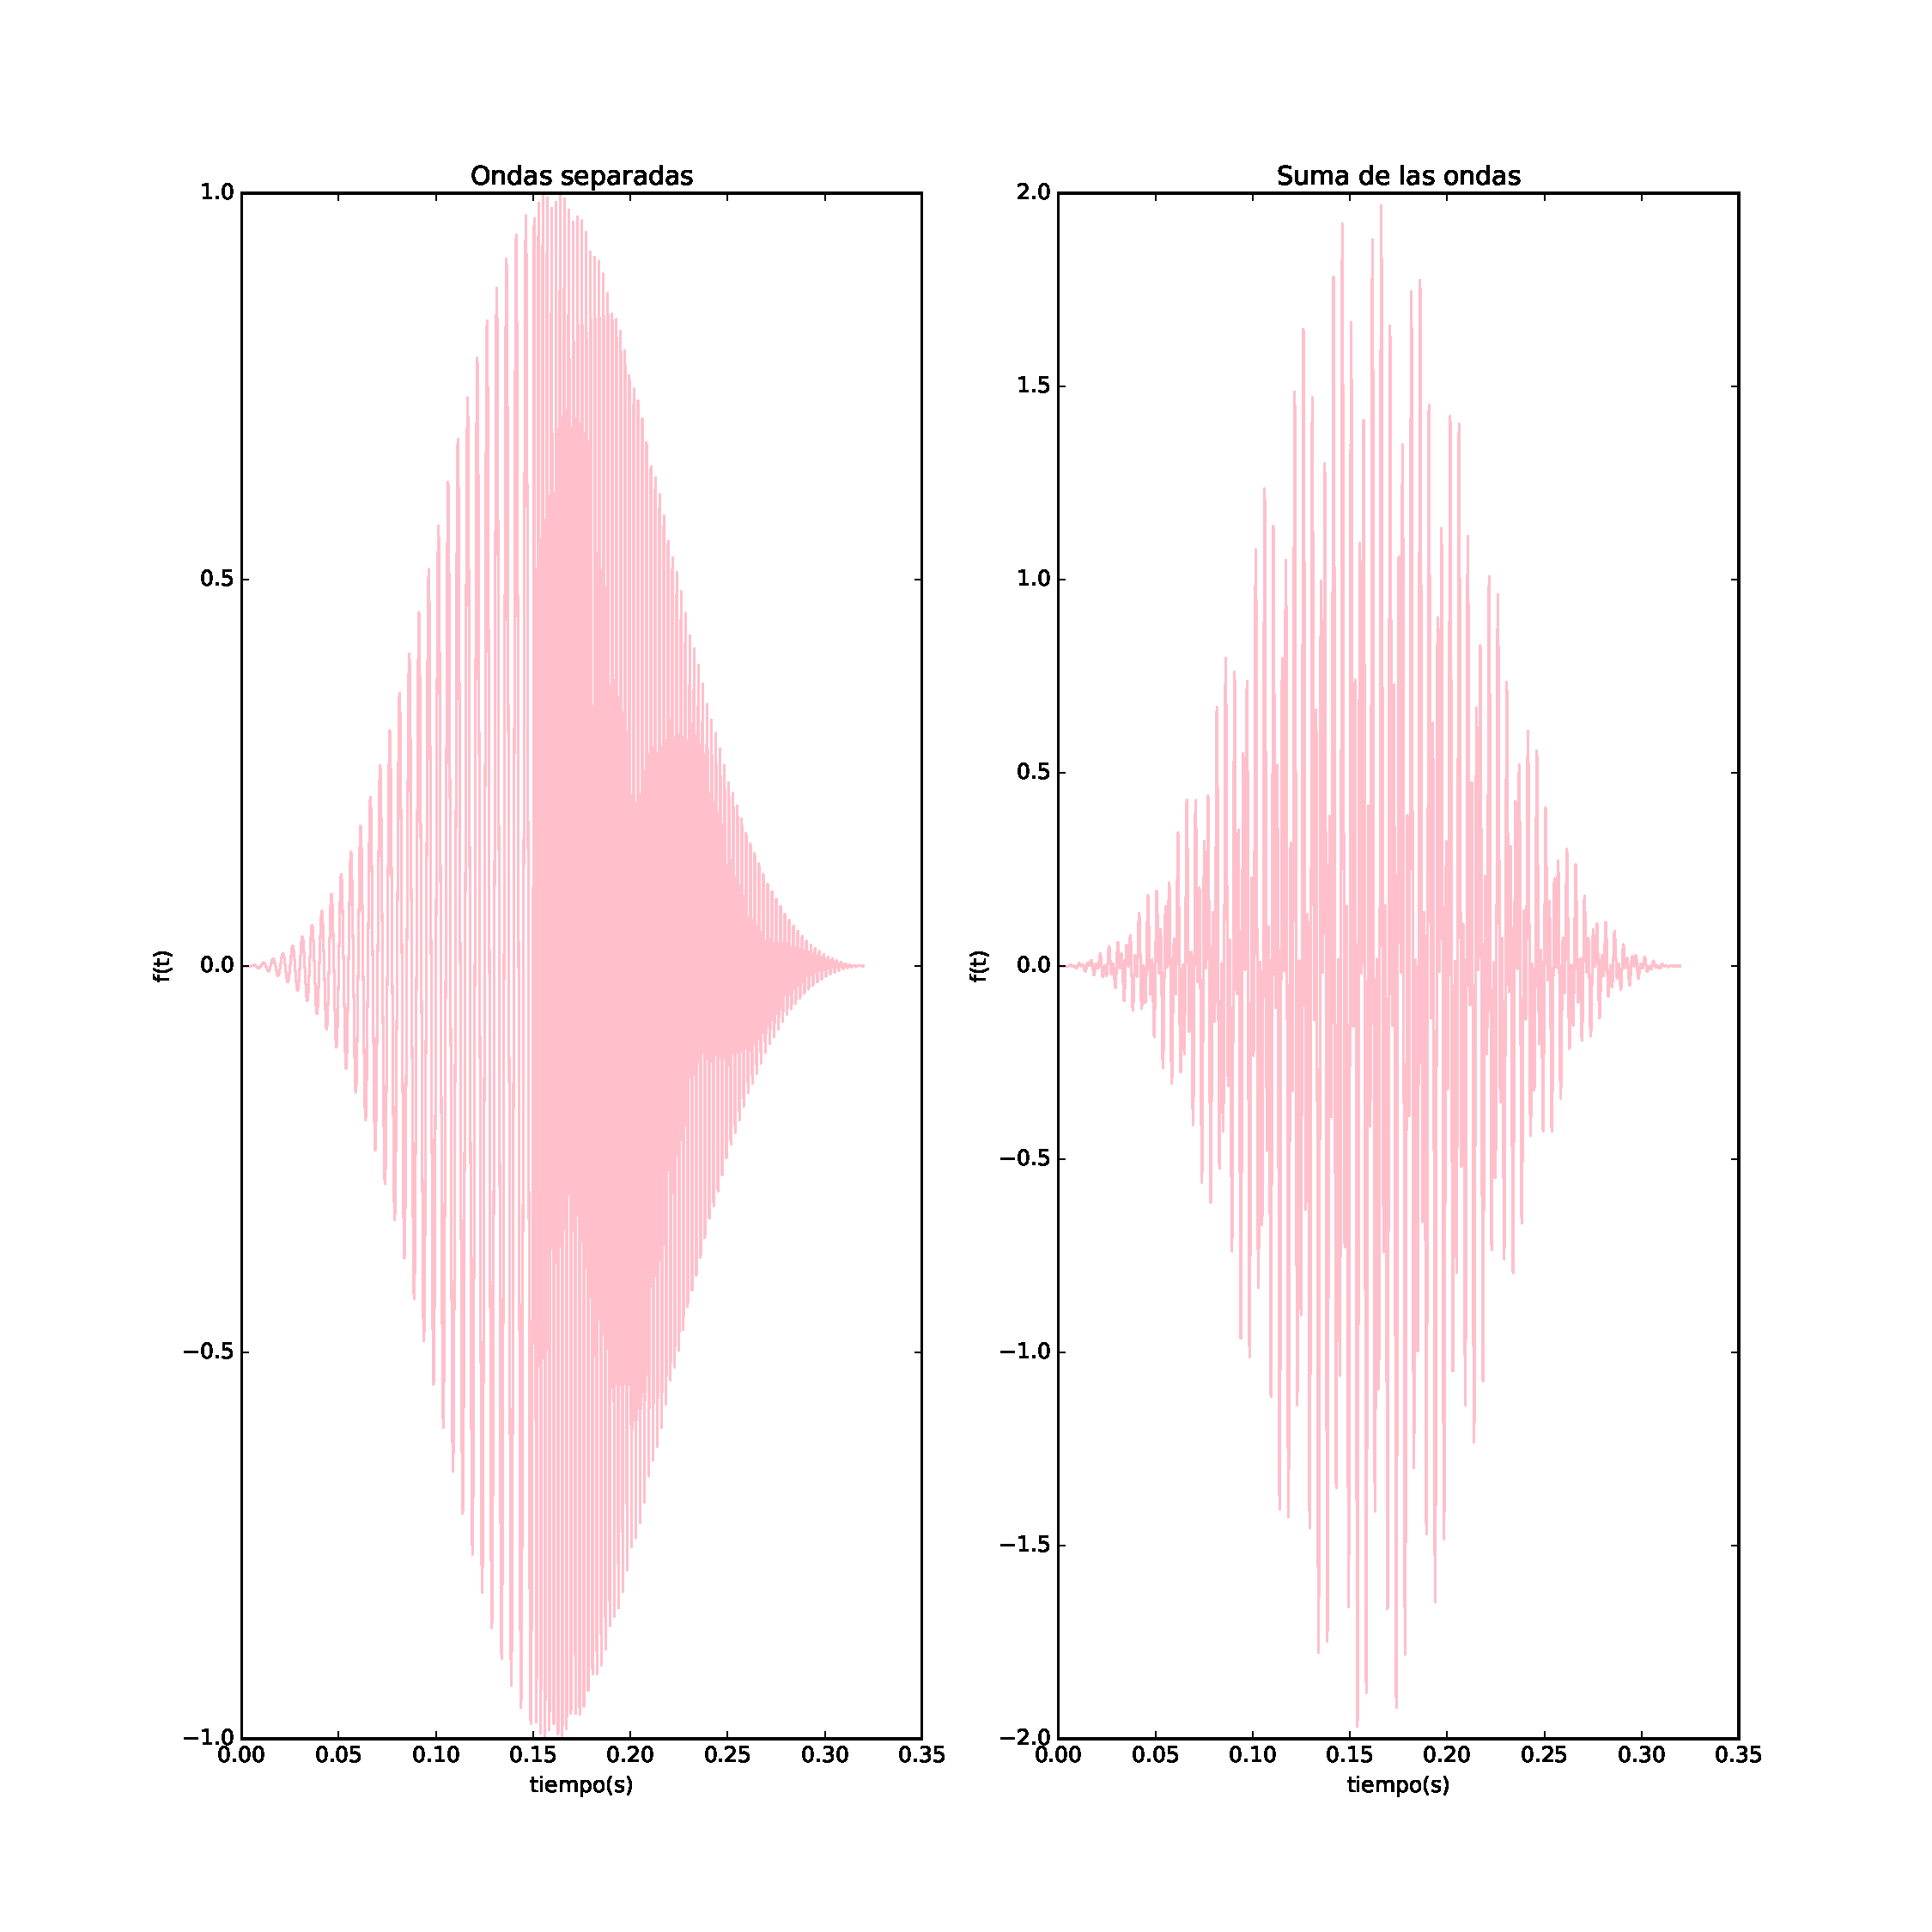
\includegraphics[width=1\textwidth]{signals.pdf}
    \caption{Grafica de las seniales.}
    \label{fig:my_label}
\end{figure}
\subsubsection{Grafica de la transforma de fourier para las seniales}
\begin{figure}[H]
    \centering
    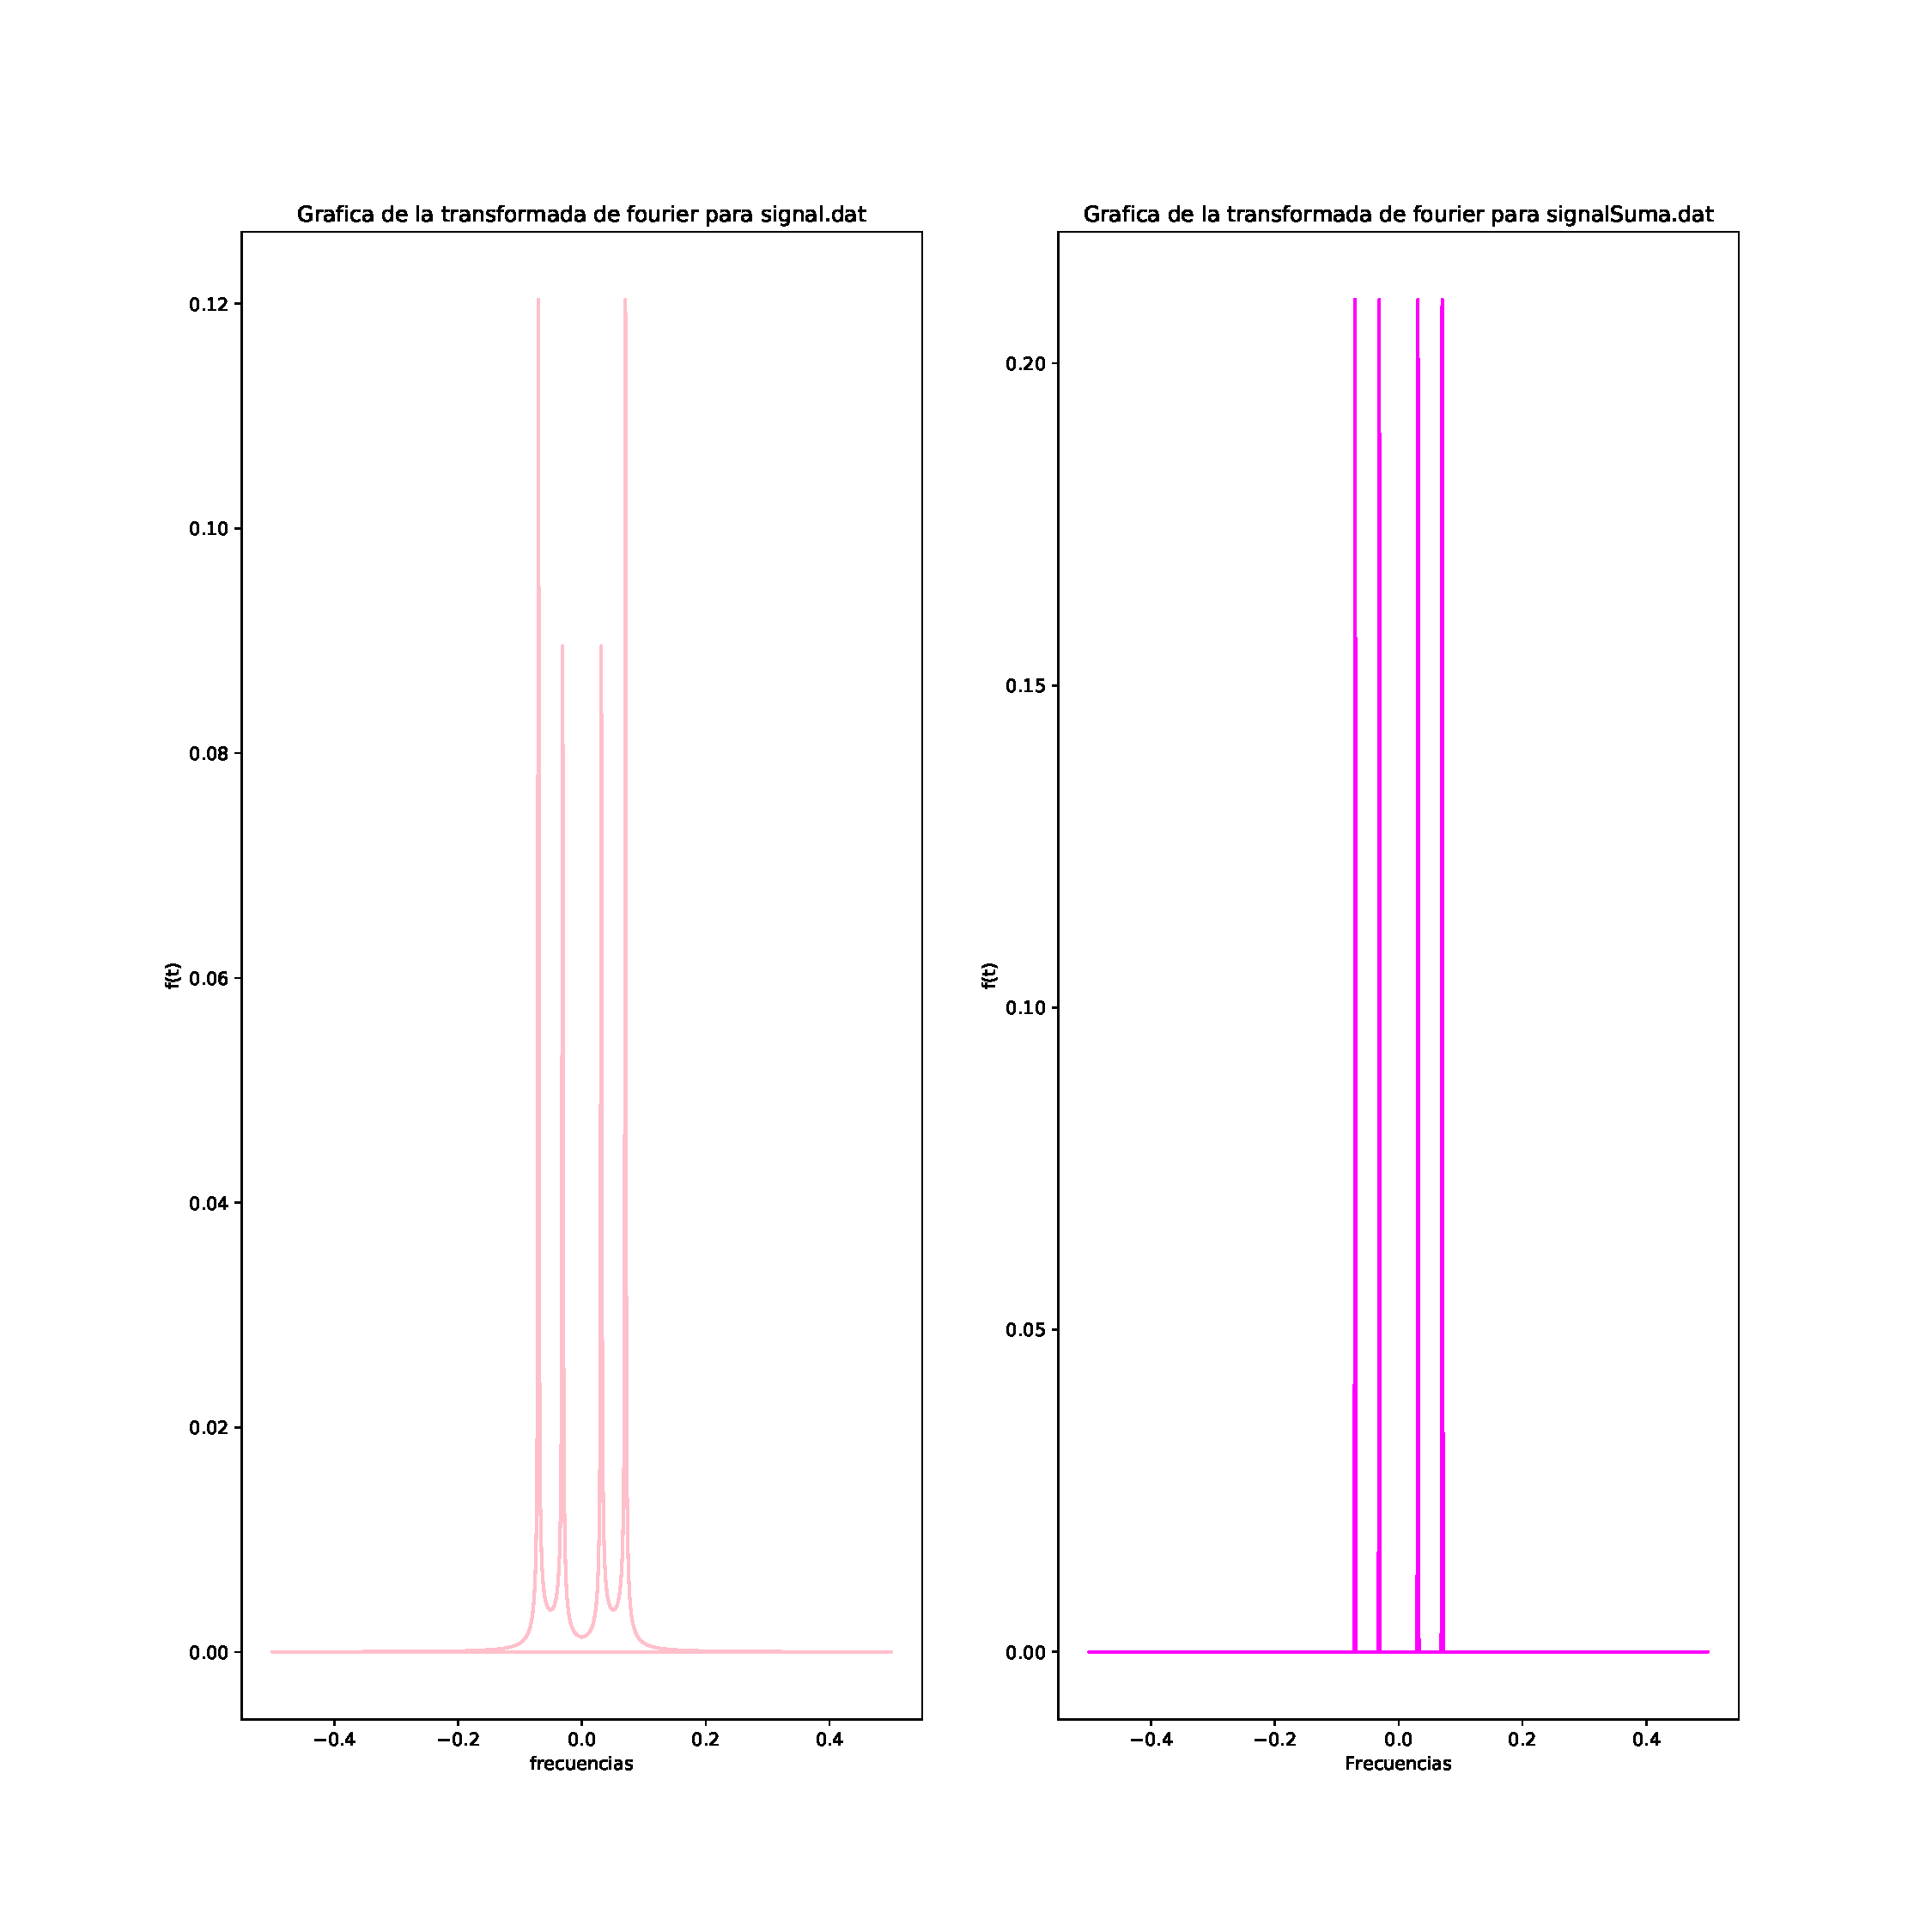
\includegraphics[width=1\textwidth]{Fourier_trans.pdf}
    \caption{Grafica de las transformadas de fourier para las dos primeras seniales.}
    \label{fig:my_label}
\end{figure}
\subsubsection{Espectograma}
\begin{figure}[H]
    \centering
    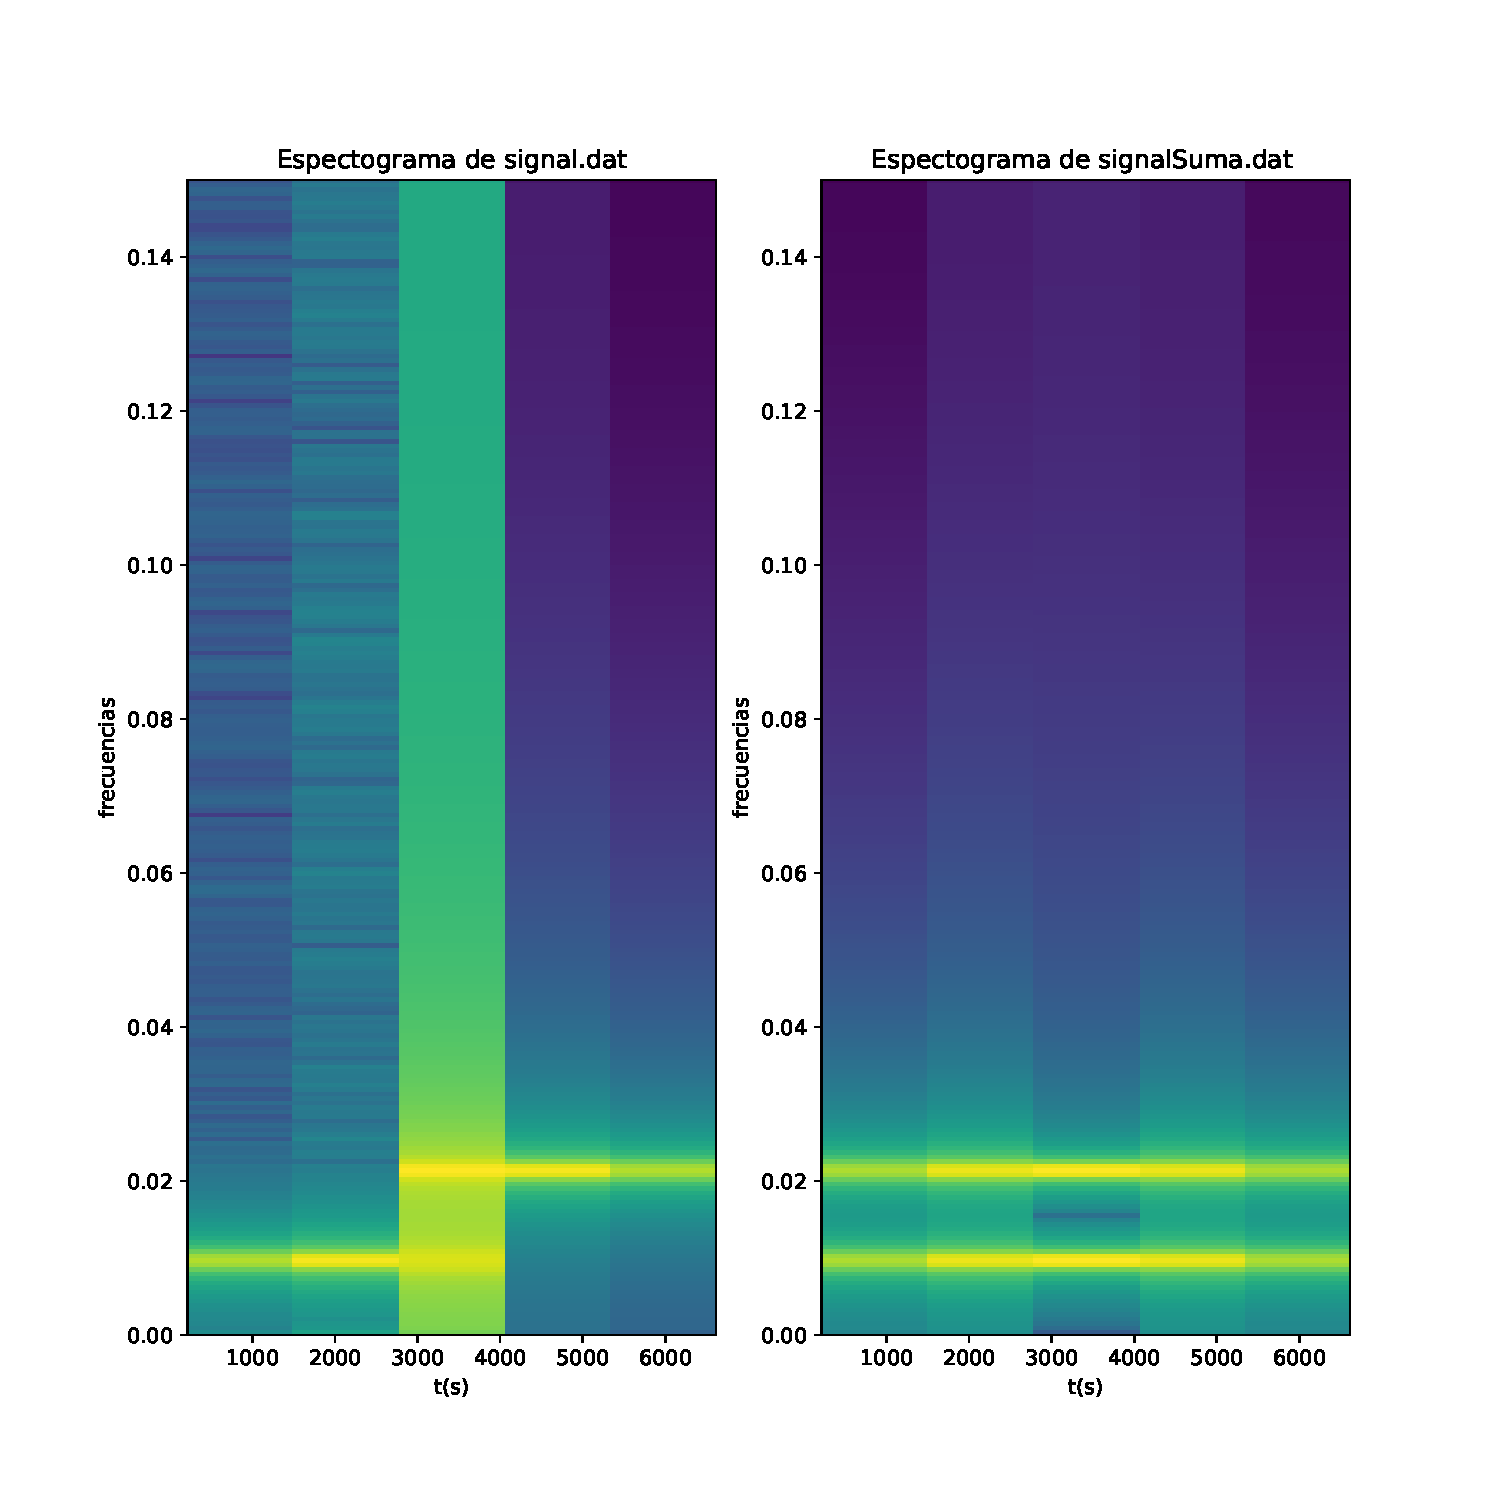
\includegraphics[width=1\textwidth]{espectograma.pdf}
    \caption{Espectogramas de las dos primeras seniales.}
    \label{fig:my_label}
\end{figure}
\subsection{Temblor.txt:}
\subsubsection{Grafica general}
\begin{figure}[H]
    \centering
    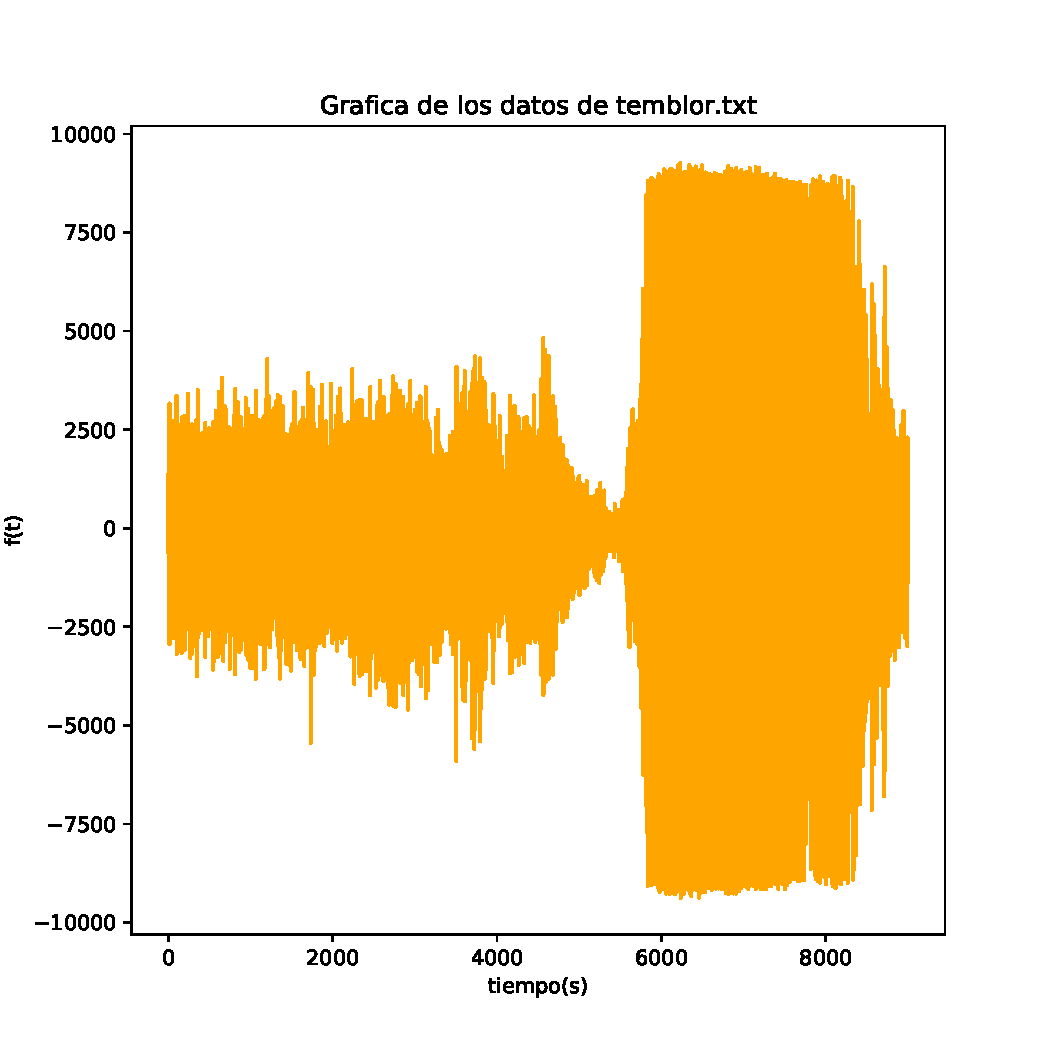
\includegraphics[width=1\textwidth]{Temblor.pdf}
    \caption{Grafica de los datos de temblor.txt}
    \label{fig:my_label}
\end{figure}
\subsubsection{Grafica transformada de fourier}
\begin{figure}[H]
    \centering
    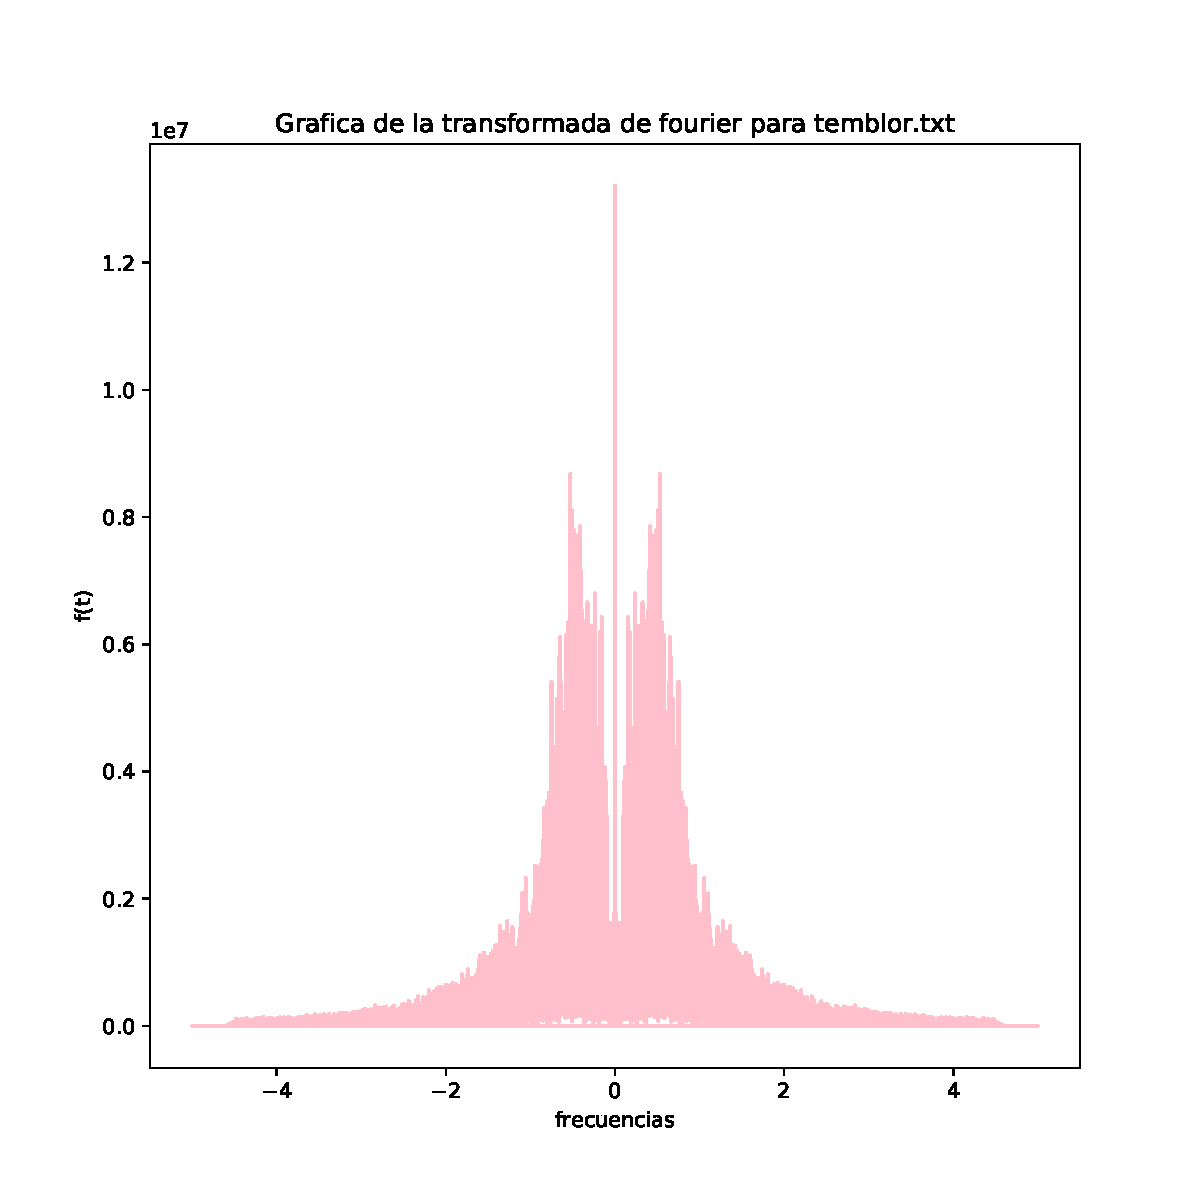
\includegraphics[width=1\textwidth]{Fourier_temblor.pdf}
    \caption{Grafica de las transformada de fourier de los datos de temblor.txt}
    \label{fig:my_label}

\end{figure}
\subsubsection{Espectograma}
\begin{figure}[H]
    \centering
    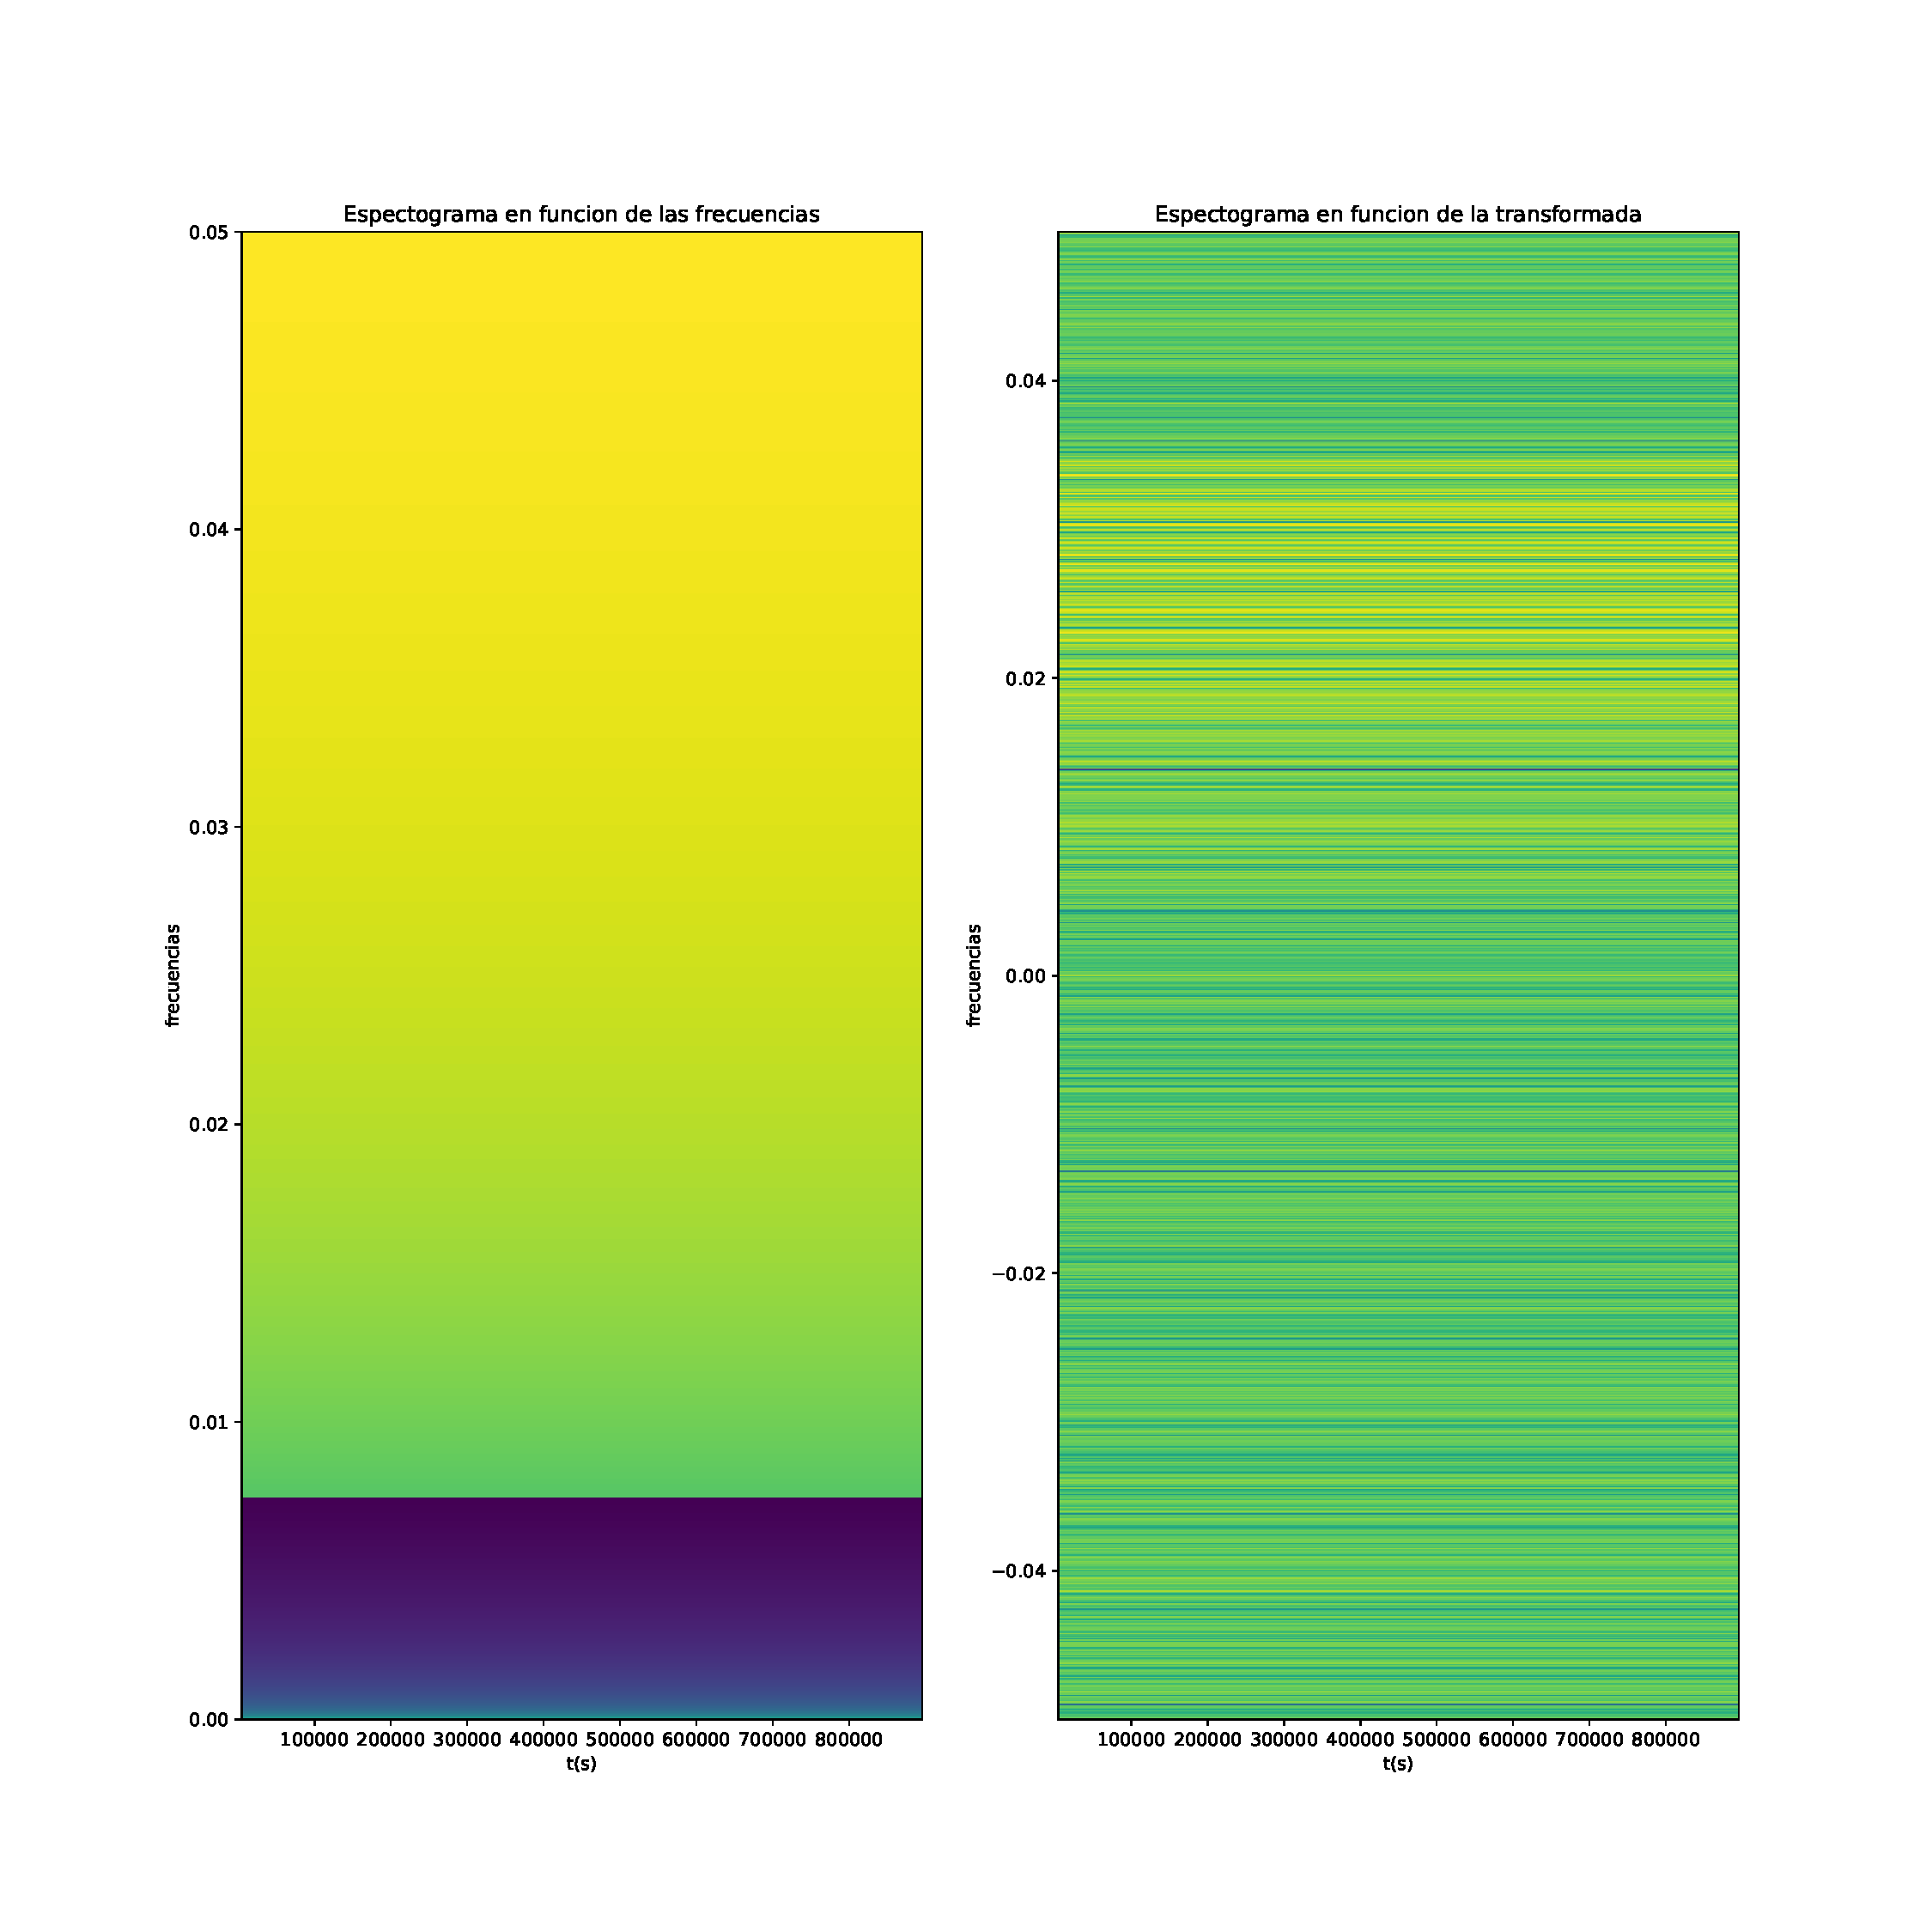
\includegraphics[width=1\textwidth]{espectograma_temblor.pdf}
    \caption{Espectograma del temblor}
    \label{fig:my_label}
\end{figure}
\section{Ejercicio 2: Ecuaciones diferenciales ordinarias}
 Debe incluir además un análisis de sus resultados. Por ejemplo hable de resonancia, del número de picos, describa las graficas de amplitudes para resonancia y no resonancia, etc....
\subsection{Primera grafica para}
\begin{figure}[H]
    \centering
    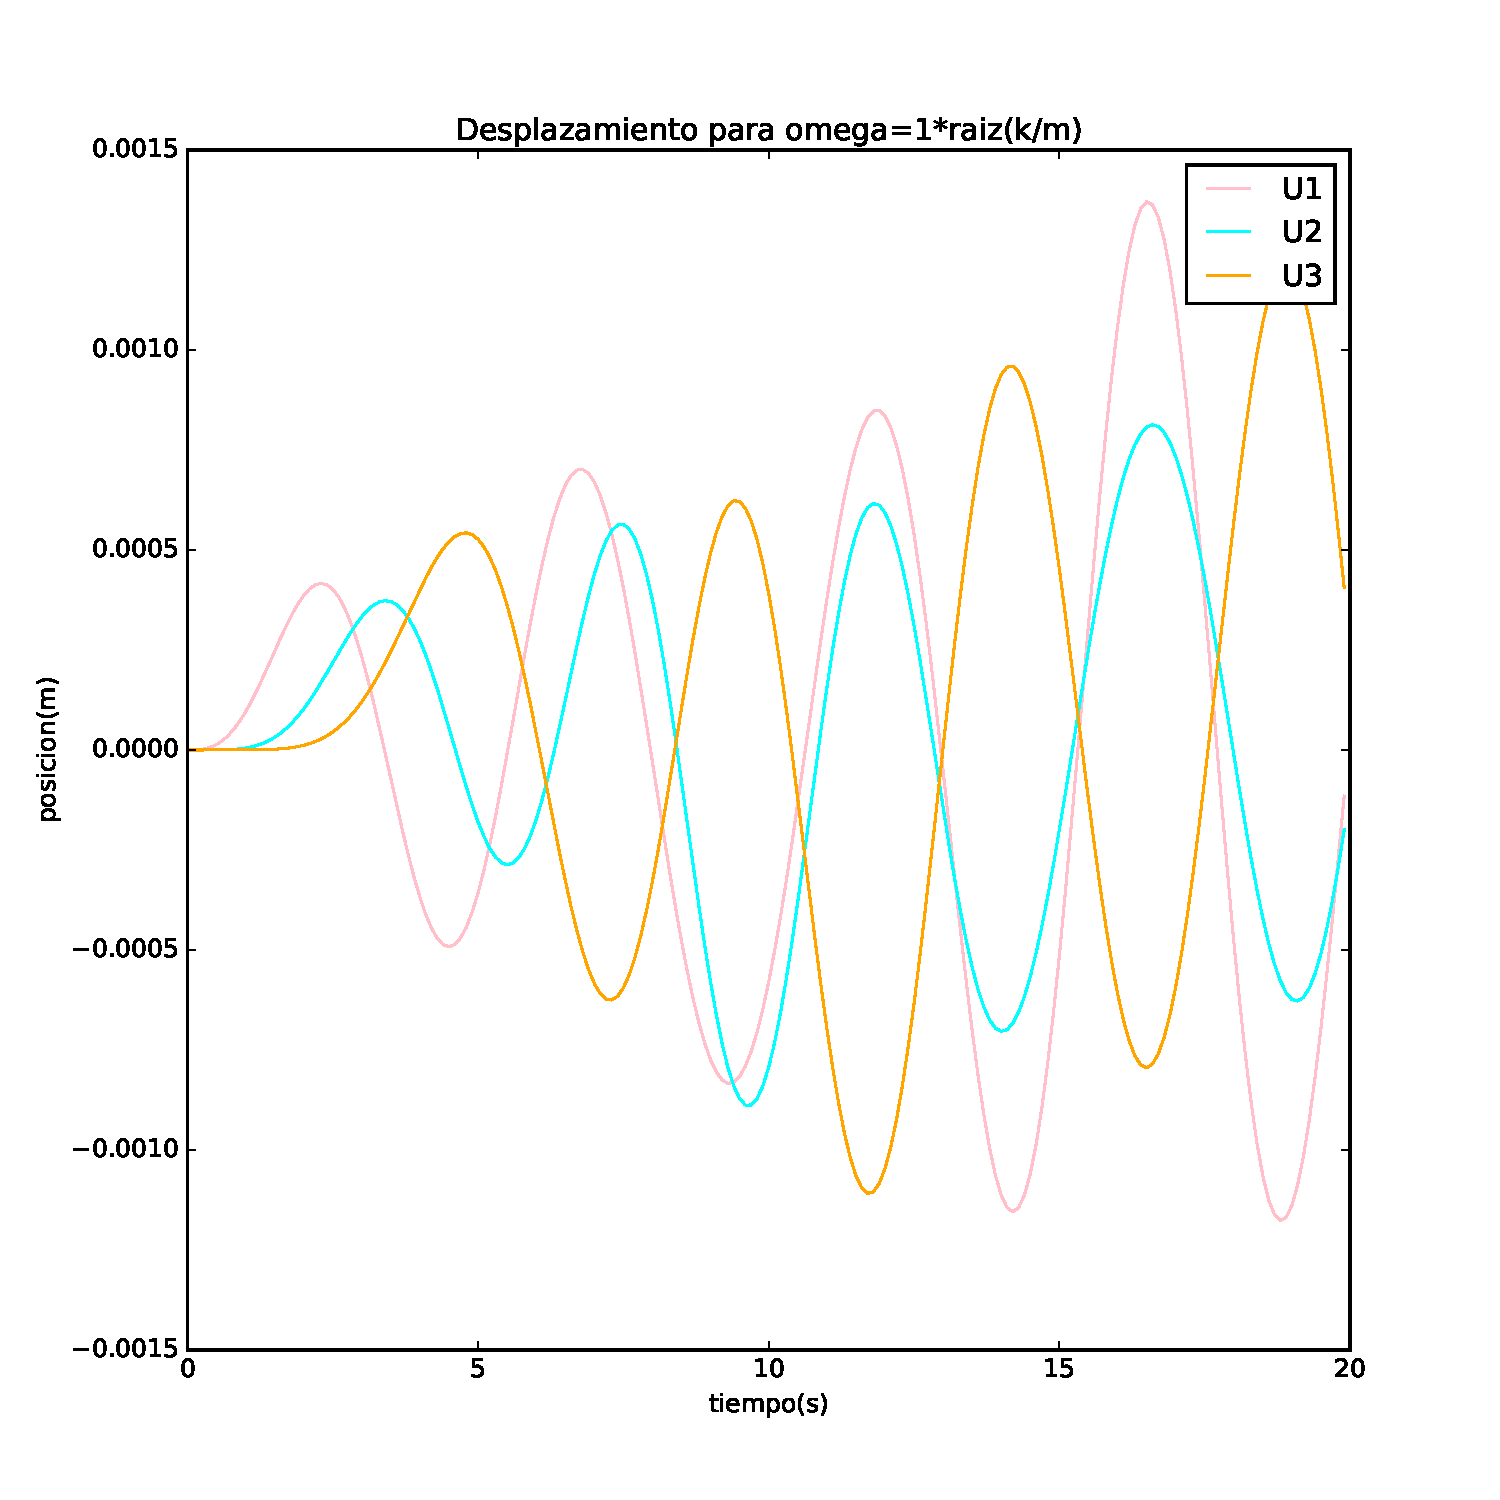
\includegraphics[width=1\textwidth]{plot_omegafijo.pdf}
    \caption{Desplazamiento del edificio en el tiempo}
    \label{fig:my_label}
\end{figure}
\subsection{Grafica de las mayores amplitudes para cada uno de los 100 omegas generados}
\begin{figure}[H]
    \centering
    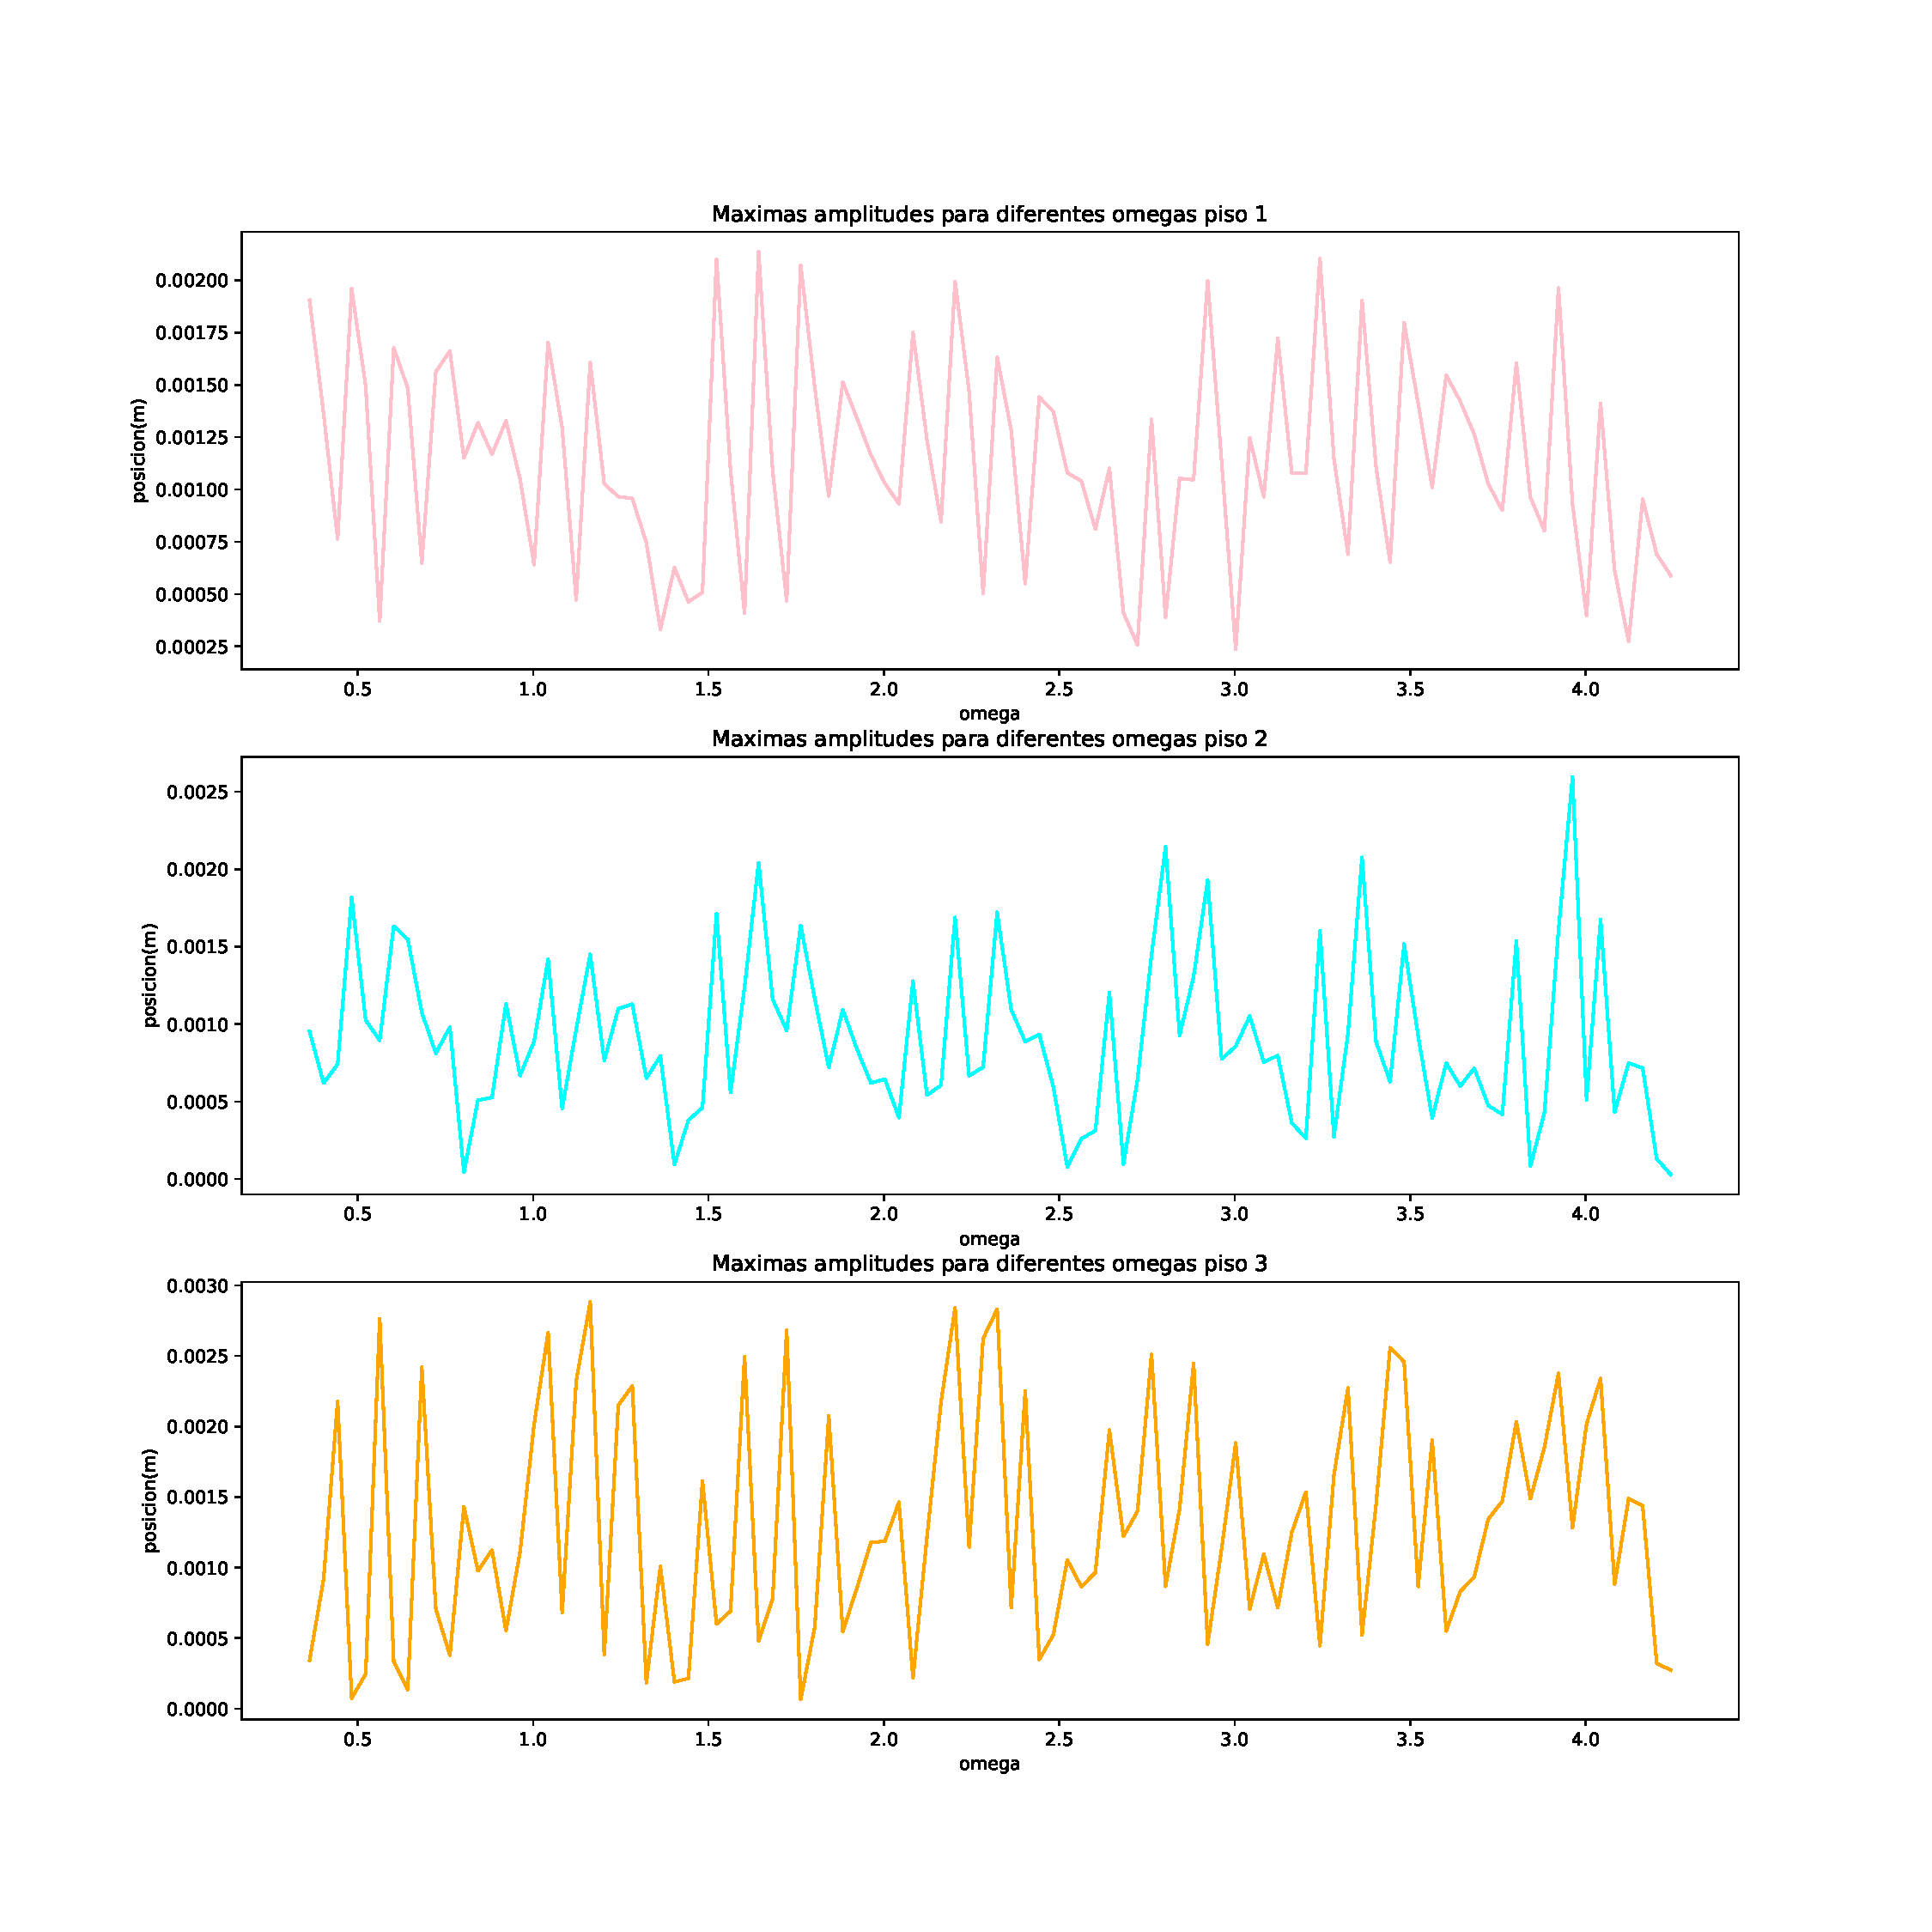
\includegraphics[width=1\textwidth]{plot_omegas.pdf}
    \caption{Mayores amplitudes para cada omega}
    \label{fig:my_label}
\end{figure}
\subsection{Grafica de los cuatro omegas}
Los omegas se escogieron al revisar la figura 8.
Estos omegas se pueden revisar tanto en Plotshw2.py como en Edificio.cpp. 
\begin{figure}[H]
    \centering
    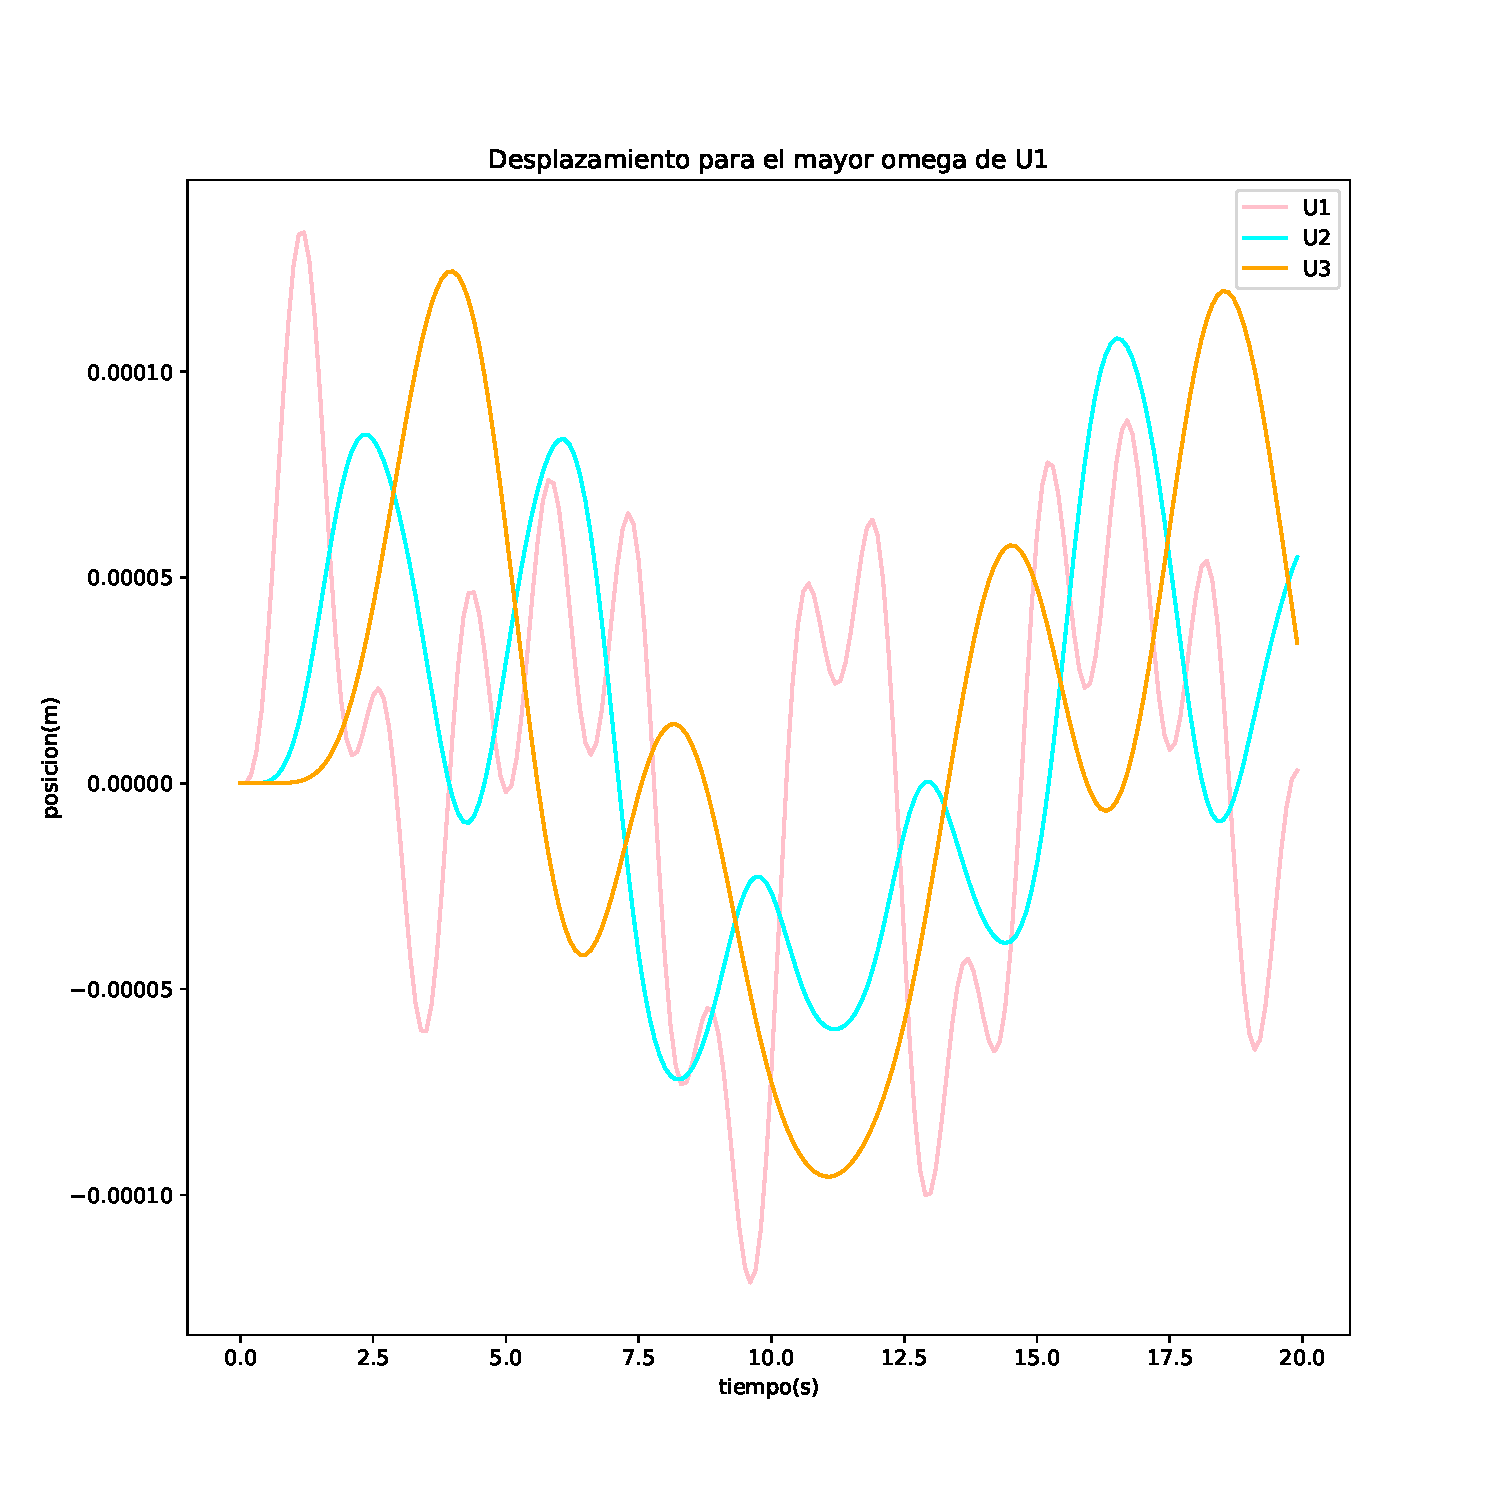
\includegraphics[width=1\textwidth]{plot_omega1.pdf}
    \caption{ Desplazamiento para omega=4.04266}
    \label{fig:my_label}
\end{figure}

\begin{figure}[H]
    \centering
    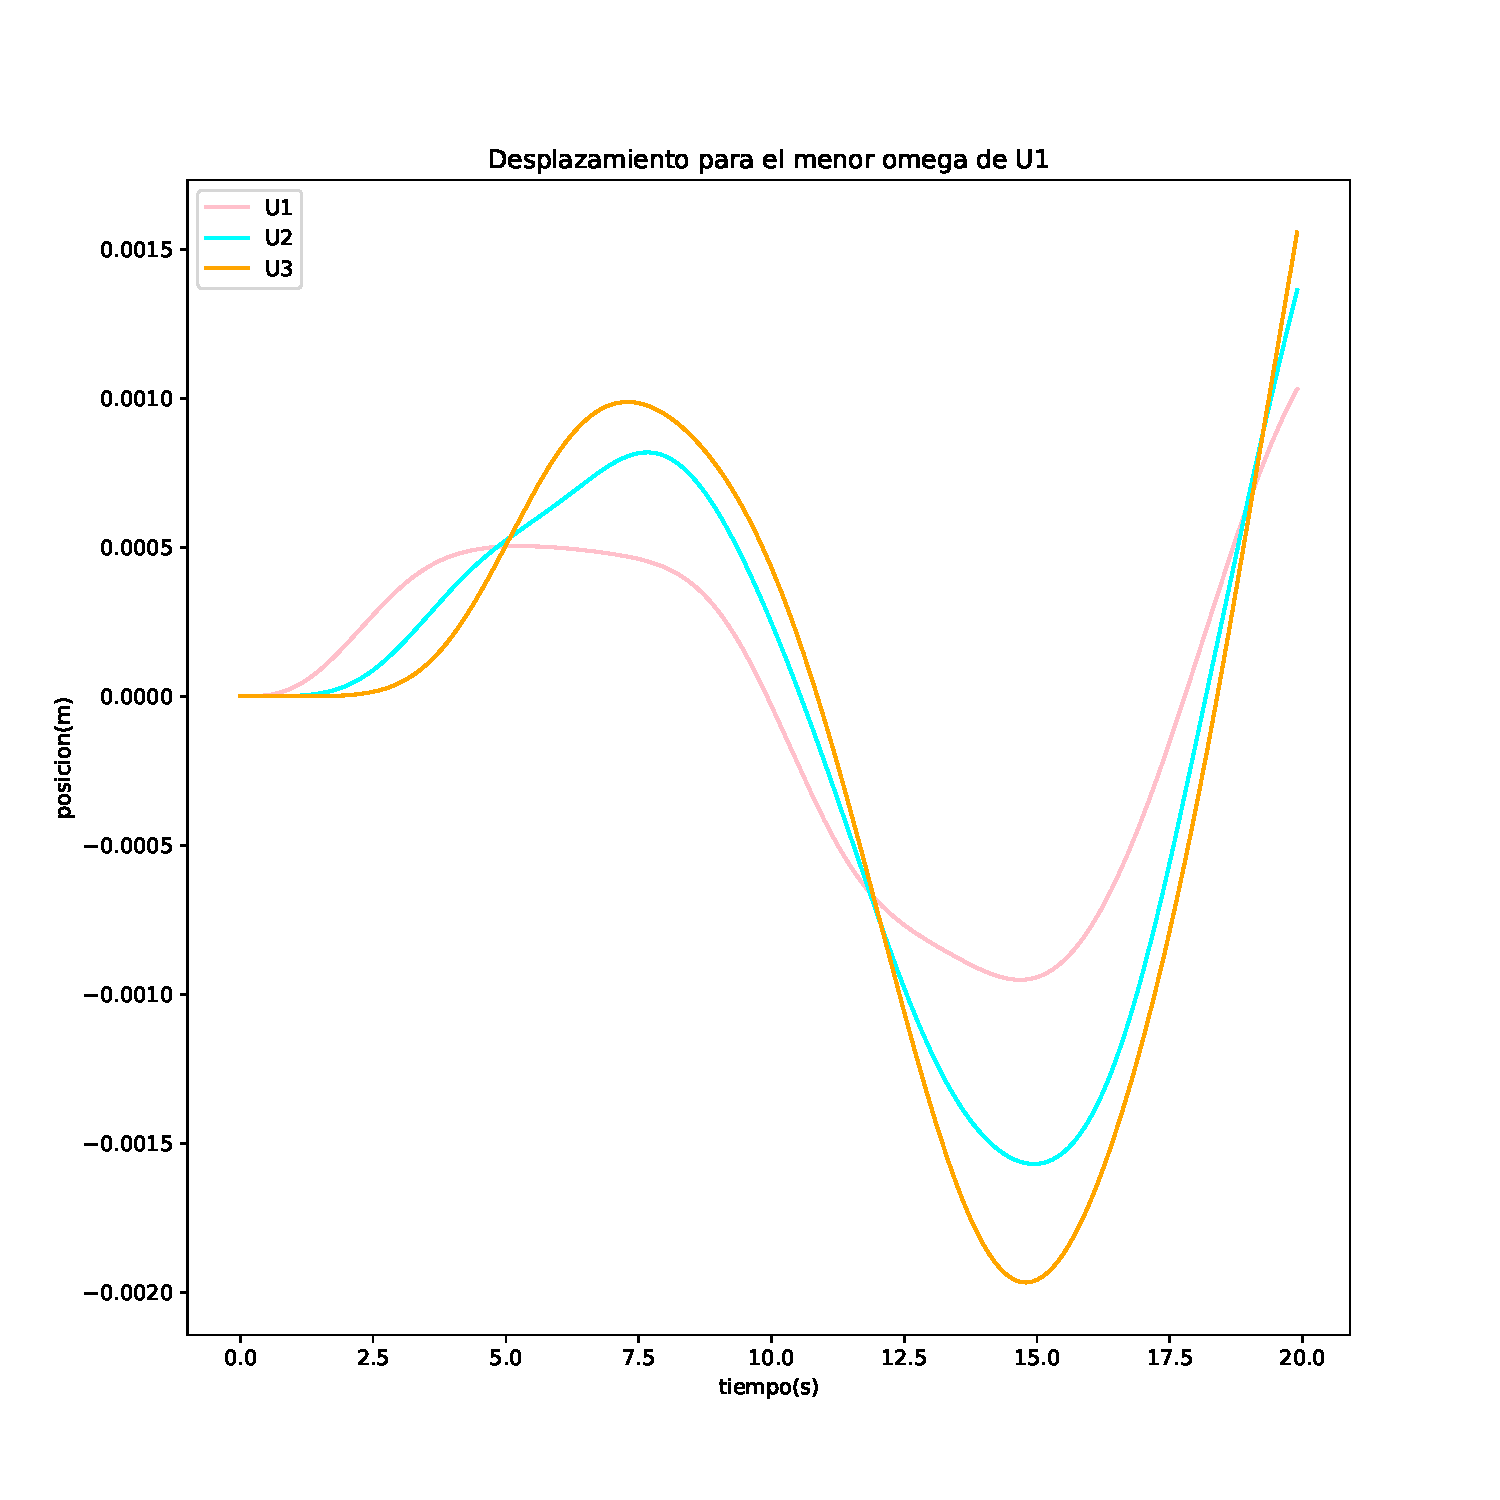
\includegraphics[width=1\textwidth]{plot_omega2.pdf}
    \caption{ Desplazamiento para omega=0.402837}
    \label{fig:my_label}
\end{figure}

\begin{figure}[H]
    \centering
    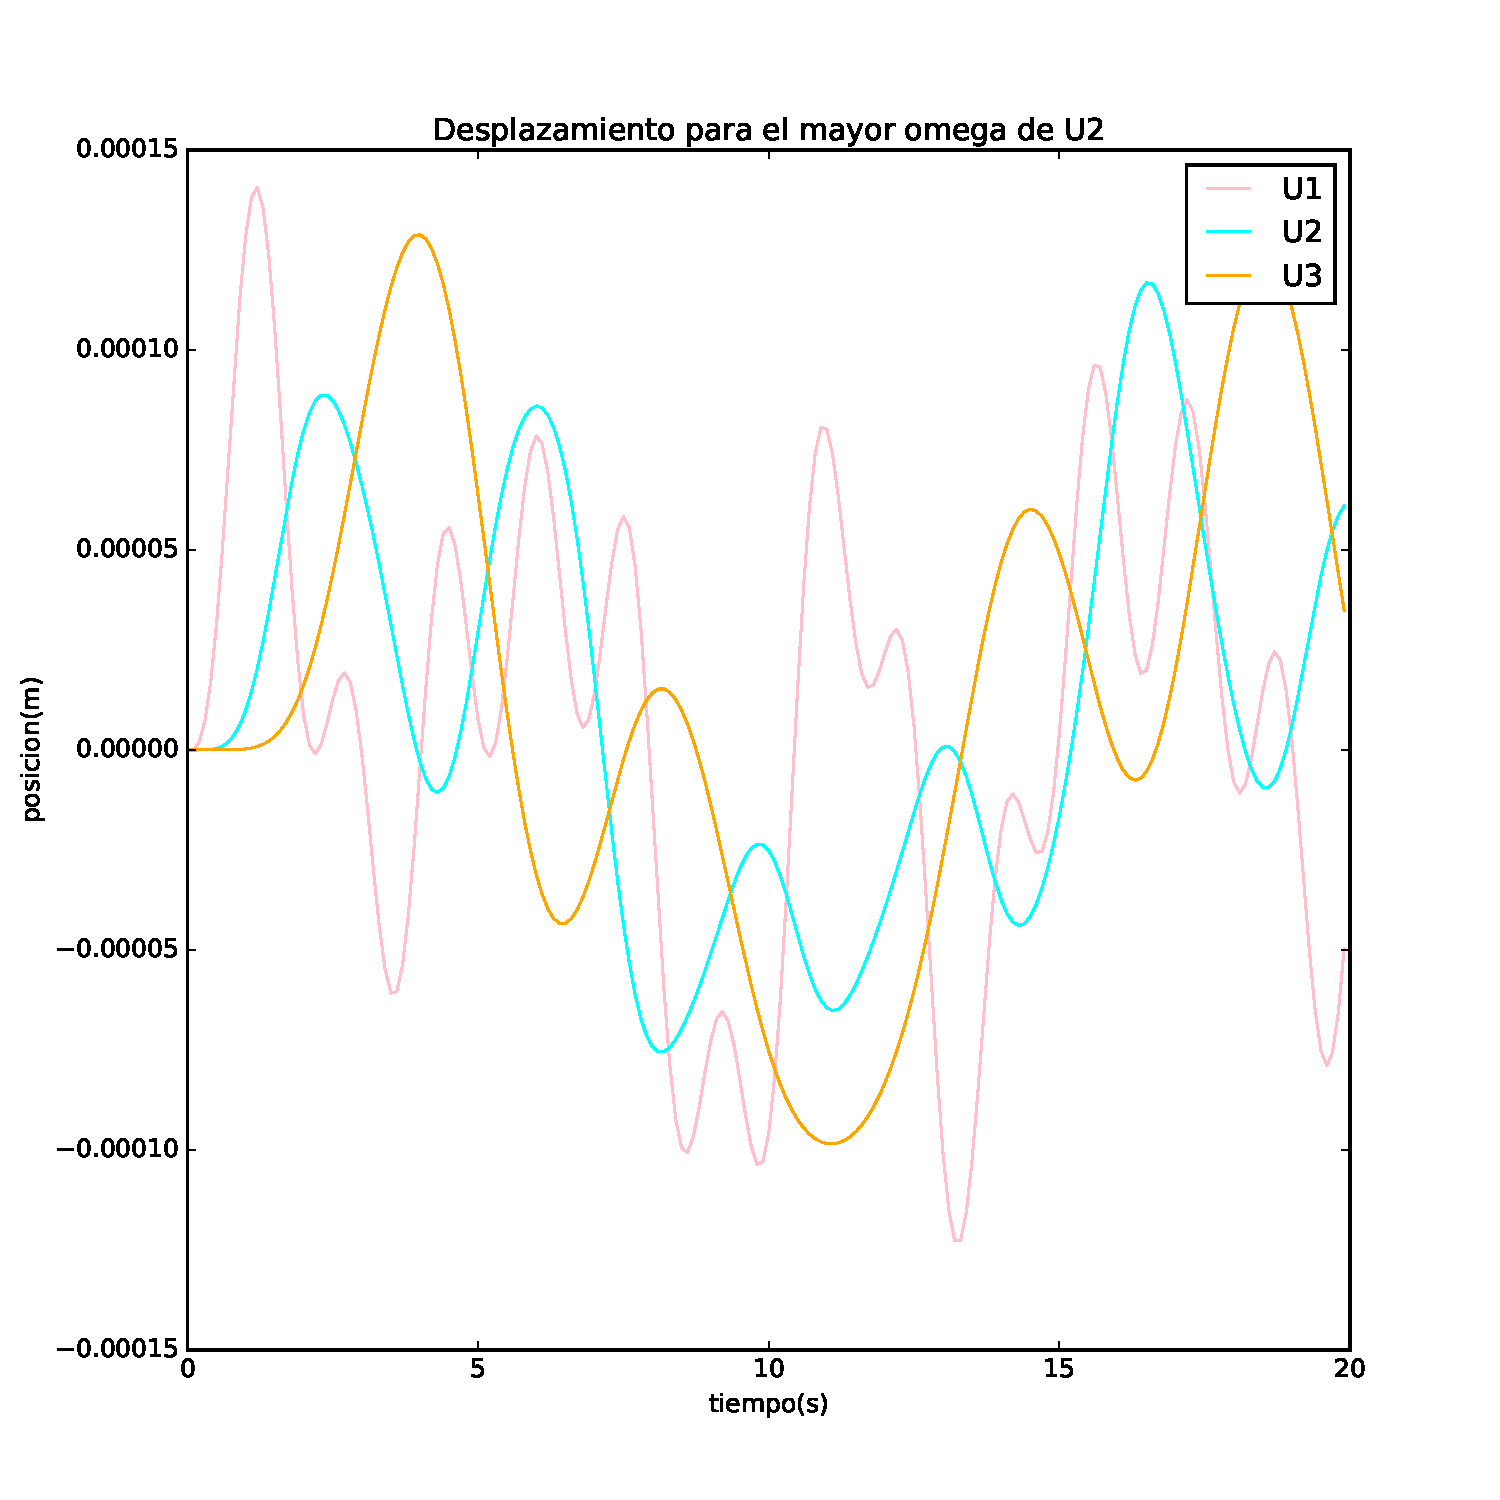
\includegraphics[width=1\textwidth]{plot_omega3.pdf}
    \caption{Desplazamiento para omega=3.92266}
    \label{fig:my_label}
\end{figure}

\begin{figure}[H]
    \centering
    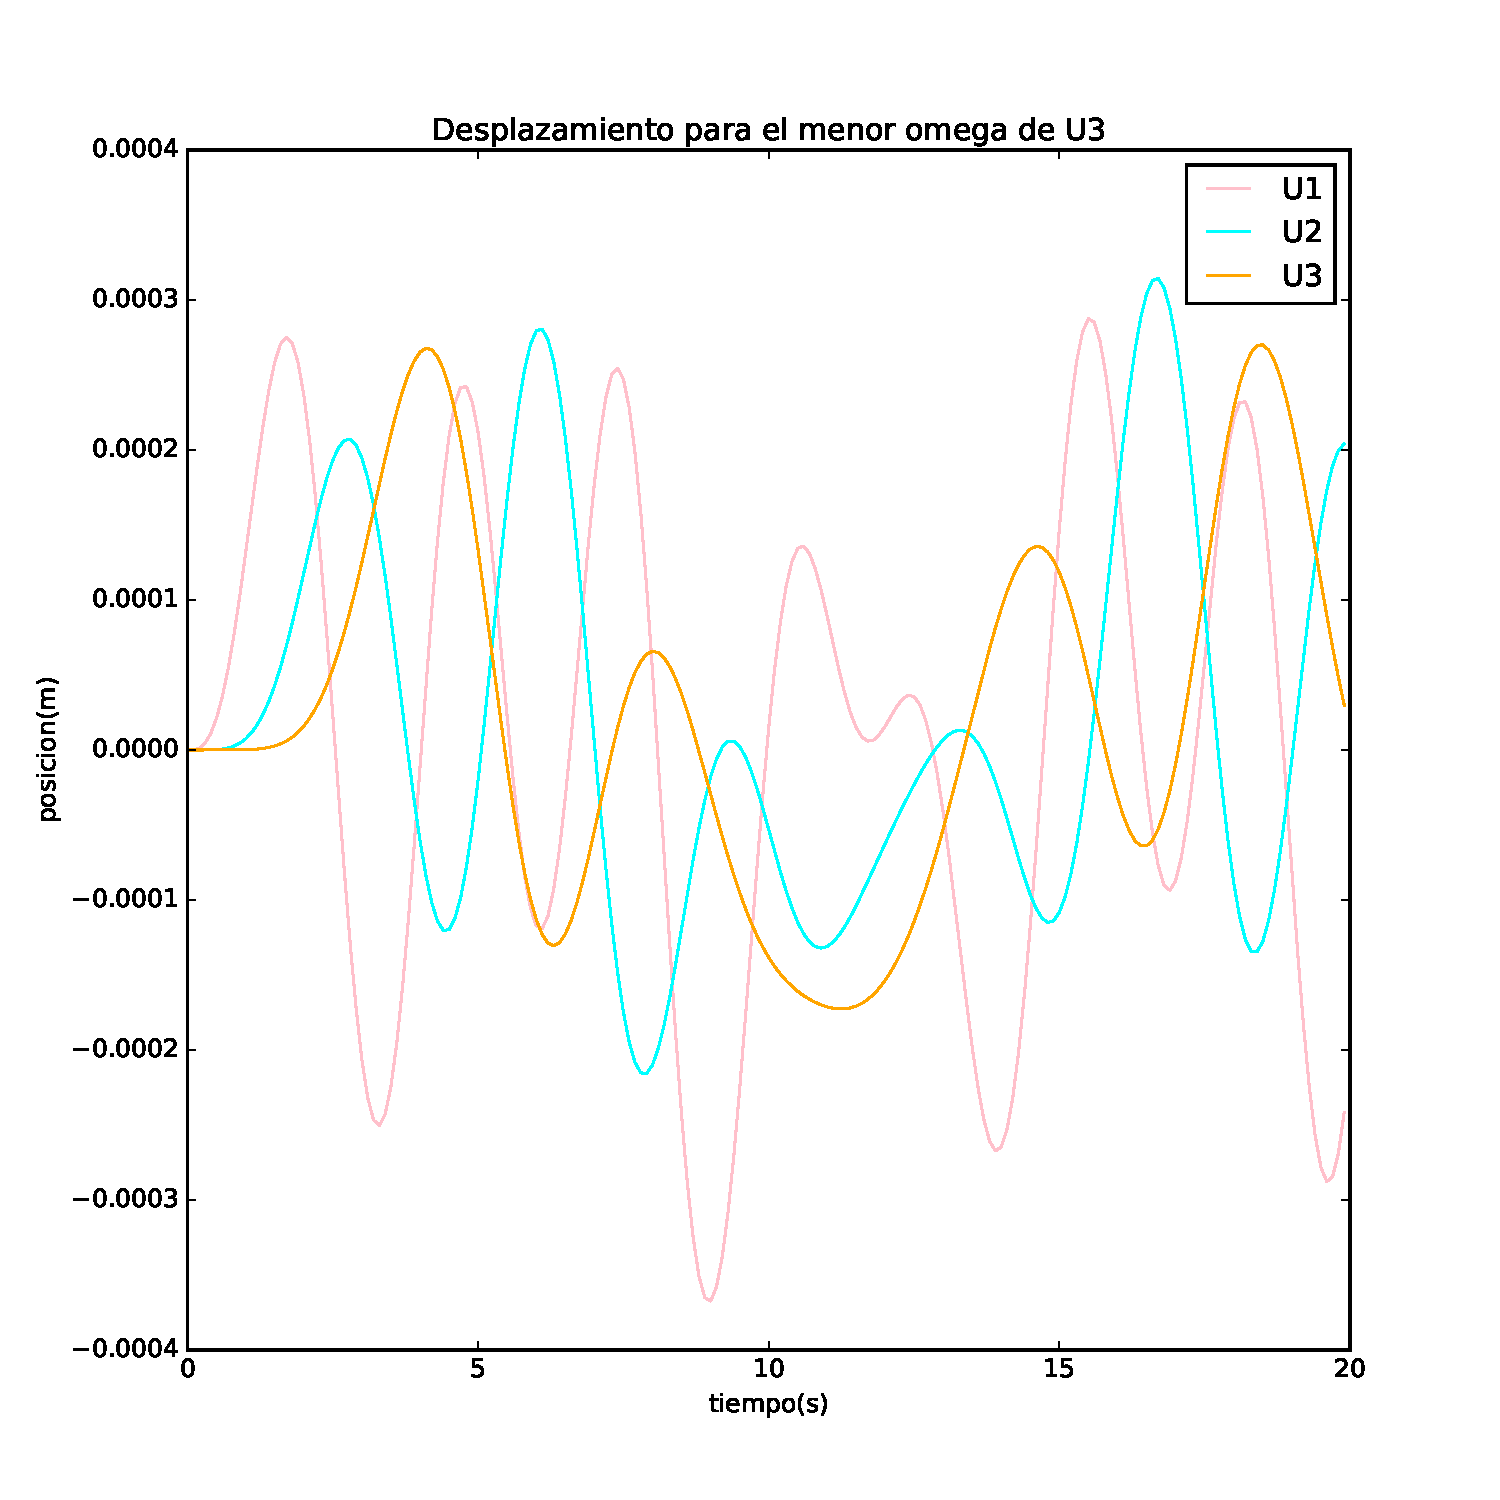
\includegraphics[width=1\textwidth]{plot_omega4.pdf}
    \caption{Desplazamiento para omega=2.32274}
    \label{fig:my_label}
\end{figure}

\end{document}